% !TeX root = ../Masterarbeit.tex

\documentclass[Masterarbeit.tex]{subfile}

\begin{document}
	
	\chapter{Results}
	
		At first, the U-net is trained with assimilations as well as masks only from the Argo era. Thus, it is set up as well as possible to reproduce argo era assimilations. The training process is then conducted until the loss parameters do not show any significant decrease anymore. Manual selection has shown that the most important loss parameters for the reconstruction of masked temperature profiles are those monitoring the direct misfit of each gridpoint and the total variation loss between neighboring gridpoints. Thus, their multiplicators have been upgraded in this version of the convolutional U-net and their development will be shown to indicate the state of training of the neural network. \\
		
		Figure \ref{fig:loss} shows the development of the hole and valid loss functions of the network training on reconstructing the first depth layer, the sea surface temperatures (SSTs). After around 1000000 training iterations, the network's loss function is not reduced significantly anymore with additional training iterations. It has reached a stable plateau. Thus, the first part of the training process is stopped and followed by 200000 iterations of finetuning. In the process of finetuning a lower learning rate of $5 \cd 10^{-5}$ ensures that the network moves as close as possible towards the local minimum it would be circling around with a higher learning rate. Figure \ref{fig:loss_val} depicts the development of the validation loss. Validation is conducted by giving the network several timesteps of one of the held back assimilation ensemble members (r2i1p1f1) to reconstruct. The resulting validation error is then calculated parallel to the training error. The progression of the validation loss shows that the network has not adjusted too much to the training data up to 1.000.000 training iterations. Thus, overfitting of the network is prevented. \\
		
		
		\section{Argo Era Reconstructions}
		
		After the training process is complete, the Argo era assimilation data of another held back ensemble member (r15i1p1f1) is masked with the corresponding observational patterns. These masks are then given to the trained neural network for reconstruction. The reconstructed temperature profiles are then converted to a timeseries of NA OHC. Figure (\ref{fig:argo_timeseries_assi}) shows this timeseries of Argo era NA OHC for both the EnKF assimilations (red) and the neural network reconstructions of masked assimilations (blue). The uncertainty range around both timeseries represents the corresponding ensemble spread. In the case of the neural network, this ensemble is produced by reconstructing the masked assimilations at different training iterations. The network state of each member is extracted 1000 iterations apart from the next. Thus, the overall state of the network is not change, but the uncertainty stemming from the exact moment of ending the training can be estimated. \\
				
		\begin{figure}[H]
			\centering
			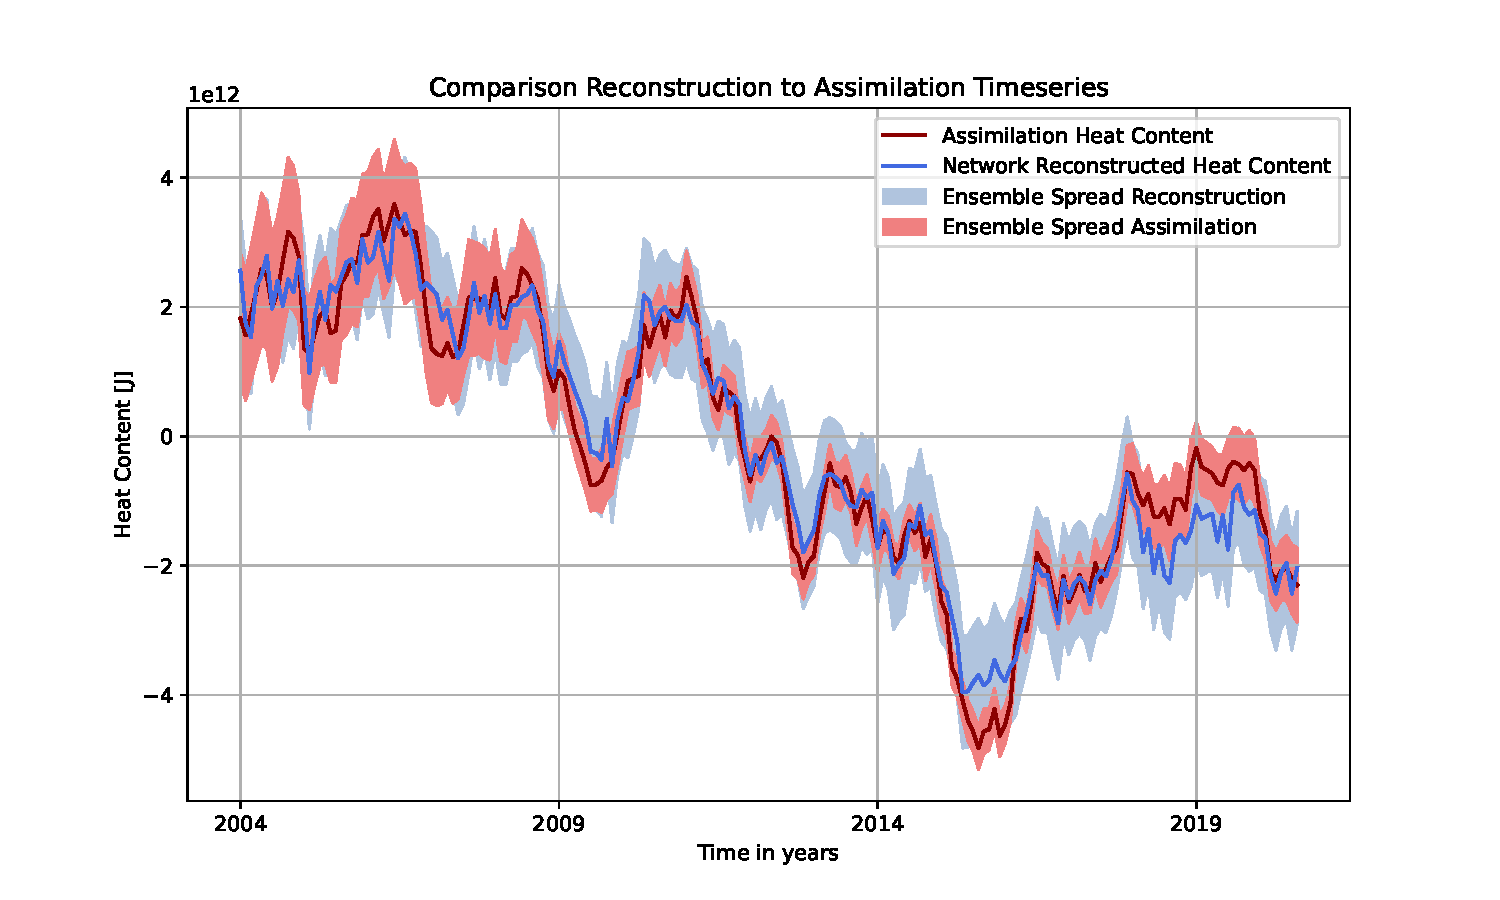
\includegraphics[width=1.0\textwidth]{../Bilder/Timeseries_argo_assi.pdf}
			\caption{Estimates of upper 700 m North Atlantic OHC of one EnKF assimilation's ensemble member (red) and the neural network reconstruction (blue). The shaded areas represent the uncertainty caused by the corresponding ensemble spread.}
			\label{fig:argo_timeseries_assi}
		\end{figure}
		
		\begin{figure}[H]
			\centering
			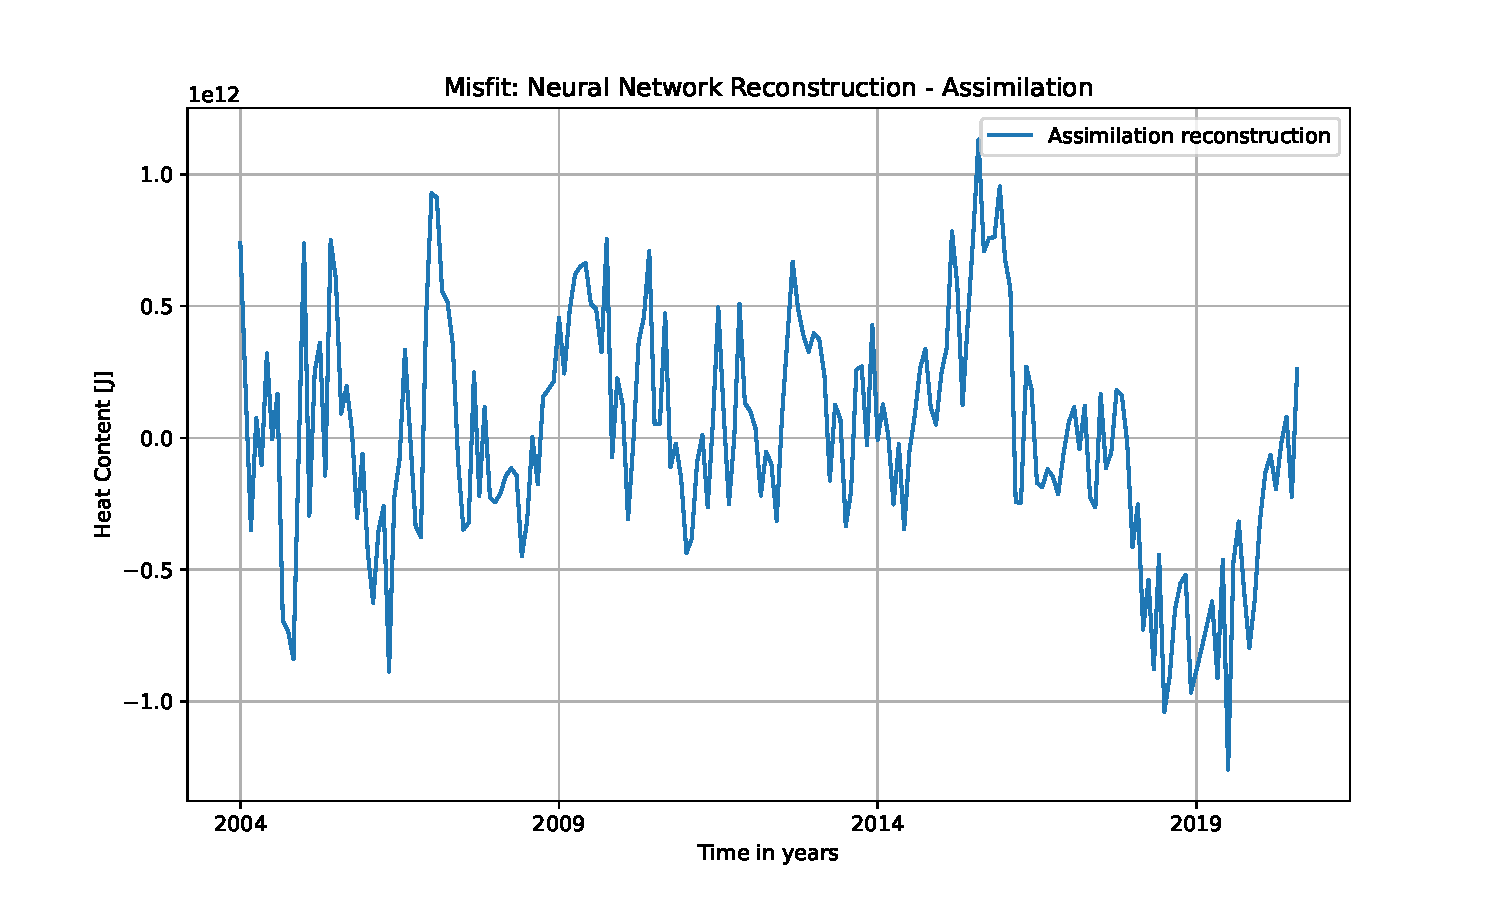
\includegraphics[width=1.0\textwidth]{../Bilder/Misfit_argo_assi.pdf}
			\caption{Misfit between EnKF assimilation NA upper 700m OHC and the neural network's reconstruction.}
			\label{fig:misfit_argo_assi}
		\end{figure}	
		
		Within the Argo era, the neural network is able to reconstruct assimilations masked with observational patterns within the assimilation's uncertainty range for monthly values. Not only do both uncertainty ranges overlap, the fit is clearly better than just inside of one standard deviation. The neural network's reconstruction even manages to capture monthly trends in the assimilation very well. Analysing this timeseries further, the misfit between both estimates shows that around 2019 the reconstruction shows a slight cool bias compared to the assimilation (\ref{fig:misfit_argo_assi}). But, as the remaining timeseries does not show any clear bias but rather just errors distributed around zero, it can be assumed to be insignificant and not a sign of a larger uncertainty within the network reconstructions. Figure \ref{fig:assi_2019} supports that assumption. It depicts NA OHC as calculated by the EnKF assimilation and the neural network for the relevant timespan from August 2018 until April 2019. The images show that no large scale bias exists during that time but that it is rather caused by several smaller scale differences in different regions. Figure \ref{fig:assi_2019} also shows that not only the network's overall OHC agrees with the EnKF assimilation, but also all major spatial OHC patterns are represented well by the neural network. The cooling of the SPG is well represented as well as the warming of the subtropical gyre (STG) and even such small scale features as the Mediterranean sea. \\
		
		\begin{figure}[H]
			\centering
			
\includegraphics[width=1.0\linewidth]{Bilder/OHC_assi_2019.pdf}
			\caption{Map of EnKF assimilation (left) and neural network reconstruction of NA upper 700m anomaly OHC estimate.}
			\label{fig:assi_2019}
		\end{figure}
		
		To further analyse the neural network's capability to capture the assimilation's spatial patterns, the pattern correlation between both OHC estimates can be taken. The pattern correlation is calculated by flattening both OHC images to a one-dimensional array and taking the anomaly correlation coefficient of both arrays. Thus, the similarities between spatial patterns for both OHC images can be estimated. Figure \ref{fig:patterncorr_assi_argo} depicts this pattern correlation during the Argo era. During the first years of the Argo era both OHC estimates show a slightly lower pattern correlation while with rising observations during the Argo era the pattern correlation reaches a constant value of over 0.8. The first 5 years also show higher month-to-month variability in pattern correlation. This can also be attributed to the higher inconsistencies in data coverage during the first years of the Argo project. \\
		
		\begin{figure}
			\centering
			
\includegraphics[width=1.0\linewidth]{Bilder/Pattern_corr_assi_argo}
			\caption{Pattern correlation for monthly estimates of anomaly NA OHC of one EnKF assimilation ensemble member and neural network reconstructions of masked assimilations.}
			\label{fig:patterncorr_assi_argo}
		\end{figure}
	
		\section{Depth Training}
		
		These first results were produced by training 20 separate neural networks, one for each depth step, and combining the results after training to calculate the overall OHC. This process does not allow for cross connections between the layers. Alternatively, the different depth steps can also be inserted into adjoining input channels of one neural network, thus also allowing for the neural network to from vertical connections in the temperature profile. This approach will from here on out be called \textit{depth training}. The additional connections incorporated in \textit{depth training} also introduce a multitude of new degrees of freedom. Thus, the neural network requires a lot more time to train as well as higher computational resources. Nonetheless, this approach of training a neural network to reconstruct the entire temperature profiles should be considered, if it yields higher correlation to the assimilation in time as well as in space. Figure \ref{fig:argo_timeseries_assi_depth} shows the OHC timeseries produced by this new reconstruction, again compared to the EnKF assimilation. \\
		
		
		The comparison shows that the depth training produces an OHC estimate with significantly lower correlation to the assimilation. Similarly, the pattern correlation between both estimates is lower for the entire timespan (\ref{fig:patterncorr_assi_argo_depth}). 
		
	
	
	
	
	
	
	
\end{document}